\documentclass[a4paper,12pt]{article}
\usepackage[ngerman]{babel}
\usepackage{multirow}
\usepackage{xltxtra}
\usepackage[utf8x]{inputenc}
\usepackage{fontspec}
\usepackage{eurosym}
\usepackage{graphicx}
\usepackage[paper=a4paper,left=25mm,right=25mm,top=25mm,bottom=25mm]{geometry}
\usepackage{makecell}
\usepackage[table]{xcolor}
\usepackage{float}
\usepackage[normalem]{ulem}
\usepackage{xcolor,colortbl}
\definecolor{Gray}{gray}{0.85}
\usepackage[automark]{scrlayer-scrpage}
\usepackage[
	colorlinks=true,
	urlcolor=blue,
	linkcolor=green
]{hyperref}
\setlength{\parindent}{0em}
\setlength{\parskip}{1ex}
\pagestyle{scrheadings}
\clearscrheadfoot
\usepackage[defaultsans]{droidsans}
\renewcommand*\familydefault{\sfdefault}
\begin{document}
\input{theme.tex}
\input{version.tex}
\newcommand{\combineDivisions}{Hinweis: Wenn weniger als 5 Teams in einer der
Altersgruppen angemeldet sind, hat die Veranstaltungsleitung die Möglichkeit,
Altersgruppen zusammenzulegen. }

\newcommand{\declareExhibition}{Wenn insgesamt weniger als 5 Teams angemeldet
sind kann die Veranstaltung zur Ausstellung erklärt werden. }

\newcommand{\robotRequirements}{Autonomer Roboter, basierend auf einer
beliebigen Plattform, der \euro{1.500} oder weniger kostet und die folgenden
Designbedingungen erfüllt, die beim Check-In überprüft werden:}


\newcommand{\tournamentScoring}{
\begin{figure}[H]
	\centering
	\def\svgwidth{\columnwidth}
	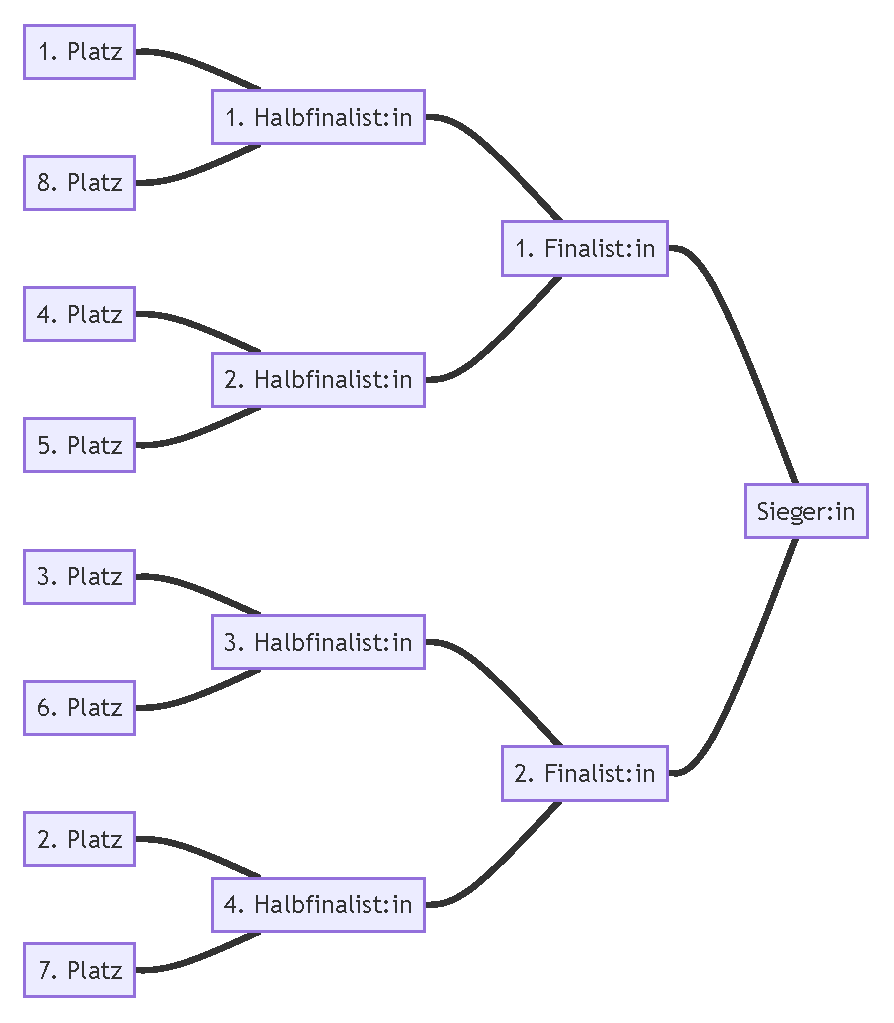
\includegraphics{tournament_score/tournament_score.pdf}
\end{figure}
}

\newcommand{\tournamentQualification}{Die aufsteigenden Teams werden
entsprechend ihrer Gesamtpunktzahl in den Turnierplan eingetragen (unten findet
ihr ein Beispiel für ein typisches Turnier mit 8 Teams). }

\newcommand{\combinedTournament}{
Hinweis: Wenn weniger als 8 Teams in allen Altersgruppen angemeldet sind, hat
die Veranstaltungsleitung die Möglichkeit, den Turnierplan entsprechend
anzupassen.
}

\newcommand{\scoreRuns}{
Die besten (8) Teams, welche am Turnier teilnehmen, werden wie folgt ermittelt:
\begin{itemize}
	\item Die Veranstaltungsleitung legt fest wieviele Läufe pro Team
		offiziell gewertet werden dürfen.
	\item Davon gehen die besten Wertungen in die Gesamtpunktzahl ein.
	\item Die Veranstaltungsleitung legt fest wieviele der offiziell
		gewerteten Läufen in die Gesamtpunktzahl eingehen.
	\item Auf Grundlage dieser Gesamtpunktzahl werden die besten Teams
		ermittelt, welche am Turnier teilnehmen.
\end{itemize}
}

\newcommand{\lightConditions}{
Die Challenge kann in Bereichen mit natürlichen Licht stattfinden, welches die
Lichtverhältnisse auf dem Spielplan verändern kann. Teams sollten darauf
vorbereitet sein, diese natürlichen Bedingungen zu meistern. }

\ohead{Regelstand: \commitDate, id: \commitID}
\title{\tagYear\ a-MAZE-ing Challenge Regeln}

\makeatletter
\let\inserttitle\@title
\makeatother
\begin{center}
	\rrgerLogo
	\huge                      % Schriftgröße einstellen
	\bfseries                   % Fettdruck einschalten
	\\
	\inserttitle
\end{center}
\section{Ziel}
Entwerfe, baue und programmiere einen Roboter, der einem erhöhten Holzlabyrinth
folgen kann, ohne herunterzufallen. Das Abschließen des Labyrinths vor dem
Zeitlimit erhöht Deine Punktzahl um Bonuspunkte.

\section{Wer kann teilnehmen?}
Teams aus 2 bis 4 Spieler:innen in \textbf{getrennten Altersgruppen}:

\begin{itemize}
	\item Grundschule (ES)
	\item Mittelstufe (MS)
\end{itemize}
\combineDivisions

\section{Anforderungen}
\robotRequirements
\begin{enumerate}
	\item Bestehen des Check-Ins durch Ausführen grundlegender operativer
		Bewegungen, wie sie in dieser Challenge benötigt werden
	\item Check-In Verfahren:
	\begin{enumerate}
		\item Der Roboter kann sich ohne externe Sensoren oder
			Fernsteuerung wie folgt bewegen:
		\begin{enumerate}
			\item eine beliebige Strecke vorwärts fahren,
			\item dann eine Drehung in eine der beiden Richtungen
				um $\approx 45^{\circ}$ oder mehr machen,
			\item sich dann um einen beliebige Strecke vorwärts
				bewegen.
		\end{enumerate}
	\end{enumerate}
	\item Der Roboter \textbf{darf keine externen Sensoren verwenden}, die
		ihm helfen, dem Labyrinth zu folgen; jedoch sind Drehgeber
		(Motor Encoder) erlaubt.
	\item Das Volumen des Roboters darf $65{.}030 \mathrm{cm}^{3}$ nicht überschreiten.
\end{enumerate}

\section{Allgemeine Spielregeln}
\begin{enumerate}
	\item \scoreRuns
	\item Der Roboter hat 2 Minuten Zeit, um das Labyrinth abzuschließen,
		wobei die Uhr von 120 Sekunden rückwärts läuft.
	\item Die Teams können nach Bedarf üben, wobei sie sich mit anderen
		übenden Teams abwechseln.
	\item Sollte die Bahn für einen offiziellen Lauf benötigt werden, geben
		die Übungsteams die Bahn ab.
\end{enumerate}

\section{Wettkampfspezifische Spielregeln}
\begin{enumerate}
	\item Wenn der Roboter aus dem Labyrinth fällt, bevor er die Ziellinie
		erreicht hat, und noch Zeit übrig ist, bringe ihn zur
		Startlinie zurück und versuche, das Labyrinth zu beenden.
	\item Ein Roboter gilt als aus dem Labyrinth gefallen, wenn eines
		seiner Räder die Oberfläche des Labyrinths \textbf{VOLLSTÄNDIG}
		nicht mehr berührt oder den Boden berührt.
\end{enumerate}

\section{Spielfeld Spezifikation}

Bahn: Alle Challenge Maße sind ungefähre Angaben.
\begin{enumerate}
	\item Alle a-MAZE-ing Strecken werden so nah wie möglich an der
		Zeichnung sein und aus Leimholz (oder einem ähnlichen lokal
		beschafften Material) von 24 cm Breite und 2 cm Höhe gebaut.
	\item Es gibt verschiedene Längen mit Kombinationen von 45, 90 und 135
		Grad Abbiegungen in beide Richtungen.
	\item Ungeachtet der Methode, mit der die Teile zusammengefügt werden,
		sollten ALLE Anstrengungen unternommen werden, um
		sicherzustellen, dass die Bahnen so glatt und frei von
		Unregelmäßigkeiten wie möglich sind.
	\item In der Altersgruppe ES gibt es 4 Geraden und 3 Abbiegungen was
		insgesamt 500 Punkte ermöglicht.
	\item In der Altersgruppe MS gibt es 6 Geraden und 5 Abbiegungen was
		insgesamt 800 Punkte ermöglicht.
	\item Abhängig vom Veranstaltungsraum und dem verfügbaren Material
		können beide Altersgruppe auf der längeren MS-Bahn betrieben
		werden. In diesem Fall befindet sich die Ziellinie der
		Altersgruppe ES irgendwo zwischen der 3. und 4. Abbiegung der
		MS-Bahn.
\end{enumerate}

\subsection{A) Material, Bahnmuster und Details zum Zusammenbau}
\begin{enumerate}
	\item Bahnmaterial: Grobspanplatten, Spanplatten, MDF,
		Mehrschichtplatte
	\item Design für die Veranstaltung: Es gibt KEIN bestimmtes Design...
		Es besteht freie Wahl, vorausgesetzt, alle 3 Abbiegungen sind
		vorhanden.
	\item Dreiecke: die Hypotenuse wird an die gerade Bahn gelegt, aus der
		sich der Roboter dreht
\end{enumerate}

\includegraphics[width=1.0\textwidth]{images/amazeing_allowed.png}

\subsection{B) Befestigung der Bahn auf dem Boden: Klebeband, 5 cm breit}

\begin{enumerate}
	\item Ausgehend vom Boden überquert das Klebeband jede
		Segmentverbindung.
	\item Beide Enden werden am Boden befestigen.
	\item Ist Oberfläche auf der Bahn \emph{NICHT} glatt?
		Nochmal neu kleben!
	\item Wertungslinie (die vorderen Räder müssen diese
		Linien berühren, um die Punkte zu erhalten)
	\begin{enumerate}
		\item Zeichne Linien durch jedes Segment
		\begin{enumerate}
			\item $\approx 20 \mathrm{cm}$ vom Ende jeder Geraden entfernt
			\item $\approx 10 \mathrm{cm}$ innnerhalb der Abbiegung
		\end{enumerate}
		\includegraphics[width=1.0\textwidth]{images/amazeing_angle.png}
	\end{enumerate}
	\item Markiere einen Bereich um jede Bahn, der NUR für die
		Spieler:innen bestimmt ist - klebe ein helles Rechteck um den
		Streckenbereich.
	\item  Ein Streckendesign - zwei Herausforderungen.
	\begin{itemize}
		\item ES - die ersten 3 Geraden + Abbiegung zur 4. Gerade
		\item MS - ganze Bahn
	\end{itemize}
	\item Abbiegung - mindestens eine $45^{\circ}$ Abbiegung UND eine (1)
		$135^{\circ}$ Abbiegung für den ES-Abschnitt
	\item Überprüfe die fertige Bahn:
	\begin{enumerate}
		\item Glattheit des Klebebandes
		\item Keine erhöhten Kanten zwischen den Brettern
	\end{enumerate}
\end{enumerate}

\section{Punktevergabe}
\begin{enumerate}
	\item Jede abgeschlossene Gerade ist 50 Punkte wert.
	\begin{enumerate}
		\item Eine Gerade gilt als abgeschlossen, wenn die Vorderräder
			die auf der Bahn markierte Wertungslinie berühren.
	\end{enumerate}
	\item Jede abgeschlossene Abbiegung ist 100 Punkte wert.
	\begin{enumerate}
		\item Eine Abbiegung gilt als abgeschlossen, wenn die
			Vorderräder die auf der Bahn markierte Wertungslinie
			berühren.
	\end{enumerate}
	\item In der Altersgruppe ES gibt es 4 Geraden und 3 Abbiegungen was
		einer Gesamtpunktzahl von 500 Punkten entspricht.
	\item In der Altersgruppe MS gibt es 6 Geraden und 5 Abbiegungen was
		einer Gesamtpunktzahl von 800 Punkten entspricht.
	\item Wenn der Roboter das Labyrinth nach Ablauf der Zeit \textbf{nicht
		beendet}, entspricht der Punktestand der weitesten
		zurückgelegten Strecke.
	\item Wenn der Roboter das Labyrinth vor Ablauf der Zeit
		\textbf{beendet}, entspricht die Punktzahl der maximalen
		Punktzahl für seine Altersgruppe, zuzüglich eines Bonus,
		bestehend aus 1 Punkt für jede verbleibende volle Sekunde.
		(z.B. wenn $3{,}14\mathrm{s}$ verbleiben, gibt es 3 Bonuspunkte.
		Bei verbleibenden $12{,}94\mathrm{s}$ gibt es 12 Bonuspunkte.
\end{enumerate}
\begin{center}
	\begin{tabular}{|c|c|c|c|c|c|} \hline
		\rowcolor{Gray}
		1. Gerade & 1. Abbiegung & 2. Gerade & 2. Abbiegung & 3. Gerade & 3. Abbiegung  \\ \hline
		50 & 150 & 200 & 300 & 350 & 450  \\ \hline
		\rowcolor{Gray}
		4. Gerade & 4. Abbiegung & 5. Gerade & 5. Abbiegung & 6. Gerade & \\ \hline
		500 (ES Ziel) & 600 & 650 & 750 & 800 (MS Ziel) & \\ \hline
	\end{tabular}
\end{center}

\section{Turnierplan}
\begin{enumerate}
	\item Die besten 8 Teams jeder Altersgruppe treten in einem Turnier
		gegeneinander an.
	\item Gleichstand wird auf der Grundlage eines vom Veranstalter
		gewählten \textbf{LEISTUNGSKRITERIUMS} aufgelöst. (Zum Beispiel:
		die höchste Einzelwertung aller gleichwertigen Teams).
        \item \tournamentQualification
	\item Die Plätze 3 und 4 werden auf der Grundlage der Ergebnisse der
		Halbfinalspiele ermittelt.
\end{enumerate}
\tournamentScoring
\combinedTournament
\end{document}
